\chapter{Results}\label{chap:results}

This chapter reports the empirical results of DCT-Page on the
benchmarks and protocol of Chapter~\ref{chap:setup}.
Section~\ref{sec:results-ruler} and Section~\ref{sec:results-longbench}
compare DCT-Page against page-based sparse-attention baselines on
long-context accuracy; Section~\ref{sec:results-speed} reports decode
throughput and a per-stage attribution of the speedup;
Section~\ref{sec:results-multipole} examines the accuracy--throughput
trade-off against the cluster-based Multipole Attention baseline; and
Section~\ref{sec:ablations} sweeps the four DCT-Page hyperparameters
that most affect accuracy and throughput.


% =====================================================================
\section{Long-Context Accuracy: RULER}\label{sec:results-ruler}
% =====================================================================

Table~\ref{tab:ruler} reports per-task RULER accuracy at 32K context
for the two base models, comparing DCT-Page against the page-based
sparse-attention baselines.  All sparse methods are run at the
$B \cdot P = 2{,}048$ selected-token budget fixed in
Section~\ref{sec:baselines}; bold entries mark the best sparse-method
score per column.

% Headline claims (from filled-in numbers below):
%   - Llama-3.1-8B: DCT-Page Avg 86.26, +5.16 vs Quest (81.10),
%     +27.28 vs InfLLM (58.98), -2.52 vs Full-KV (88.78).
%   - Qwen3-8B:     DCT-Page Avg 83.72, +6.40 vs Quest (77.32),
%     +16.98 vs SeerAttention-R (66.74), -5.11 vs Full-KV (88.83).

\begin{table}[ht]
  \centering
  \caption[RULER per-task accuracy at 32K context.]
  {RULER accuracy on 13 tasks at 32K context, in percent.  Models:
   Llama = Llama-3.1-8B-Instruct, Qwen3 = Qwen3-8B.
   Sparse methods are matched at a $2{,}048$-token selected budget.
   Task abbreviations: S = NIAH Single, MK = NIAH MultiKey,
   MV = NIAH MultiValue, MQ = NIAH MultiQuery, VT = Variable
   Tracking, CWE = Common Words Extraction, FWE = Frequent Words
   Extraction, QA = long-document question answering.
   Best sparse-method score per column in bold.}
  \label{tab:ruler}
  \centering
  \resizebox{\textwidth}{!}{%
  \scriptsize
  \setlength{\tabcolsep}{3pt}
  \begin{tabular}{l l ccc ccc cc c cc cc c}
    \toprule
    Model & Method
      & S1 & S2 & S3
      & MK1 & MK2 & MK3
      & MV & MQ
      & VT
      & CWE & FWE
      & QA1 & QA2
      & Avg \\
    \midrule
    \multirow{4}{*}{Llama}
      & Full-KV  & 100.00 & 100.00 & 100.00 & 100.00 & 96.00 & 100.00 & 98.00 & 100.00 & 98.40 & 48.40 & 93.33 & 72.00 & 48.00 & 88.78 \\
      & Quest    & \textbf{100.00} & \textbf{100.00} & \textbf{100.00} & \textbf{100.00} & \textbf{96.00} & 32.00 & 97.00 & 99.00 & \textbf{97.60} & \textbf{30.00} & 82.67 & \textbf{72.00} & \textbf{48.00} & 81.10 \\
      & InfLLM   & \textbf{100.00} & 88.00 & \textbf{100.00} & 84.00 & 12.00 & 8.00 & 75.00 & 92.00 & 44.00 & 6.40 & \textbf{93.33} & 32.00 & 32.00 & 58.98 \\
      & DCT-Page & \textbf{100.00} & \textbf{100.00} & \textbf{100.00} & \textbf{100.00} & \textbf{96.00} & \textbf{92.00} & \textbf{100.00} & \textbf{100.00} & 96.00 & 28.00 & \textbf{93.33} & \textbf{72.00} & 44.00 & \textbf{86.26} \\
    \midrule
    \multirow{4}{*}{Qwen3}
      & Full-KV         & 100.00 & 100.00 & 100.00 & 96.00 & 88.00 & 96.00 & 95.00 & 100.00 & 96.00 & 86.40 & 93.33 & 56.00 & 48.00 & 88.83 \\
      & Quest           & \textbf{100.00} & \textbf{100.00} & \textbf{100.00} & 92.00 & \textbf{88.00} & 8.00 & 90.00 & 90.00 & 98.40 & \textbf{58.80} & 84.00 & 48.00 & \textbf{48.00} & 77.32 \\
      & SeerAttention-R & \textbf{100.00} & 84.00 & 92.00 & 92.00 & 40.00 & 28.00 & 65.00 & 88.00 & 78.40 & 21.60 & \textbf{90.67} & 44.00 & 44.00 & 66.74 \\
      & DCT-Page        & \textbf{100.00} & \textbf{100.00} & \textbf{100.00} & \textbf{96.00} & \textbf{88.00} & \textbf{72.00} & \textbf{97.00} & \textbf{100.00} & \textbf{100.00} & 46.00 & 89.33 & \textbf{52.00} & \textbf{48.00} & \textbf{83.72} \\
    \bottomrule
  \end{tabular}%
  }
\end{table}


% =====================================================================
\section{Long-Context Accuracy: LongBench v1 and v2}\label{sec:results-longbench}
% =====================================================================

LongBench measures long-context performance on realistic text rather
than synthetic retrieval.  Table~\ref{tab:longbench-v1} reports
per-task scores on the six-task v1 subset (Section~\ref{sec:bench-longbench});
Table~\ref{tab:longbench-v2} reports v2 multiple-choice accuracy
broken down by difficulty (easy / hard) and by context length
(short / medium / long).

% Headline claims (from filled-in numbers below):
%   - LongBench v1: DCT-Page Avg 50.27 (Llama) / 48.63 (Qwen3),
%     within 0.05-0.07 pts of Full-KV. Best sparse method on both.
%   - LongBench v2 (Overall): DCT-Page beats Full-KV.
%     Llama:  30.02 vs 29.82 (+0.20 over Full-KV; best sparse method).
%     Qwen3:  32.01 vs 29.64 (+2.37 over Full-KV; SeerAttention-R
%             slightly higher at 32.60).
%   - Quest collapses on Medium/Long context cells of v2
%     (Long: 0.00 / 0.93 for Llama / Qwen3).

\begin{table}[ht]
  \centering
  \caption[LongBench v1 per-task scores.]
  {LongBench v1 scores on six representative tasks.  Models:
   Llama = Llama-3.1-8B-Instruct, Qwen3 = Qwen3-8B.  Metrics are
   per-task official metrics (F1 for QA, ROUGE-L for summarization,
   accuracy for in-context learning).  Best sparse-method score per
   column in bold.}
  \label{tab:longbench-v1}
  \centering
  \footnotesize
  \setlength{\tabcolsep}{4pt}
  \begin{tabular}{l l c c c c c c c}
    \toprule
    Model & Method
      & NarrativeQA & Qasper & MFQA-en
      & 2WikiMQA & GovReport & TriviaQA
      & Avg \\
    \midrule
    \multirow{4}{*}{Llama}
      & Full-KV  & 29.24 & 45.37 & 54.99 & 45.33 & 35.34 & 91.65 & 50.32 \\
      & Quest    & 28.99 & 43.08 & 51.25 & 44.80 & 29.97 & 91.98 & 48.35 \\
      & InfLLM   & 25.80 & 43.89 & 49.41 & \textbf{46.47} & 34.70 & \textbf{92.07} & 48.72 \\
      & DCT-Page & \textbf{29.50} & \textbf{45.96} & \textbf{55.08} & 44.68 & \textbf{35.04} & 91.34 & \textbf{50.27} \\
    \midrule
    \multirow{4}{*}{Qwen3}
      & Full-KV         & 24.98 & 48.32 & 51.85 & 43.14 & 33.46 & 90.48 & 48.70 \\
      & Quest           & \textbf{25.47} & 45.74 & 50.74 & 43.15 & 31.20 & 90.30 & 47.77 \\
      & SeerAttention-R & 25.30 & 47.13 & 50.85 & \textbf{43.33} & 32.54 & 90.31 & 48.24 \\
      & DCT-Page        & 24.93 & \textbf{48.01} & \textbf{51.93} & 42.89 & \textbf{33.54} & \textbf{90.48} & \textbf{48.63} \\
    \bottomrule
  \end{tabular}
\end{table}

\begin{table}[ht]
  \centering
  \caption[LongBench v2 accuracy.]
  {LongBench v2 multiple-choice accuracy (\%) broken down by
   difficulty and context-length category.  Models:
   Llama = Llama-3.1-8B-Instruct, Qwen3 = Qwen3-8B.  Best
   sparse-method score per column in bold.}
  \label{tab:longbench-v2}
  \centering
  \footnotesize
  \setlength{\tabcolsep}{5pt}
  \begin{tabular}{l l c c c c c c}
    \toprule
    Model & Method
      & Overall
      & Easy & Hard
      & Short & Medium & Long \\
    \midrule
    \multirow{4}{*}{Llama}
      & Full-KV  & 29.82 & 30.21 & 29.58 & 35.00 & 26.05 & 28.70 \\
      & Quest    & 18.29 & 22.40 & 15.76 & \textbf{38.33} & 10.70 & 0.00 \\
      & InfLLM   & 26.04 & 25.52 & 26.37 & 31.67 & \textbf{26.05} & 16.67 \\
      & DCT-Page & \textbf{30.02} & \textbf{33.33} & \textbf{27.97} & 34.44 & \textbf{26.05} & \textbf{30.56} \\
    \midrule
    \multirow{4}{*}{Qwen3}
      & Full-KV         & 29.64 & 31.25 & 28.62 & 28.70 & 26.98 & 33.33 \\
      & Quest           & 18.09 & 21.88 & 15.76 & 38.33 & 9.77 & 0.93 \\
      & SeerAttention-R & \textbf{32.60} & \textbf{36.46} & 30.23 & \textbf{38.89} & \textbf{30.23} & \textbf{26.85} \\
      & DCT-Page        & 32.01 & 33.33 & \textbf{31.19} & \textbf{38.89} & 28.84 & \textbf{26.85} \\
    \bottomrule
  \end{tabular}
\end{table}


% =====================================================================
\section{Decode Throughput and Per-Stage Profile}\label{sec:results-speed}
% =====================================================================

This section reports decode-time speedup of DCT-Page over Full-KV at
five context lengths $L \in \{8, 16, 32, 64, 128\}\text{K}$ tokens and
two batch sizes (1, 2), measured under the protocol of
Section~\ref{sec:speed-protocol}.
Figure~\ref{fig:speedup} shows the speedup curves;
Table~\ref{tab:per-stage} decomposes the attention-time budget into
the per-stage components defined in Section~\ref{sec:speed-protocol}.

% TODO (headline claims to substantiate):
%   - 5.65x attention-only speedup at 128K (batch 1).
%   - 1.70x end-to-end speedup at 128K (batch 1).

\begin{figure}[ht]
  \centering
  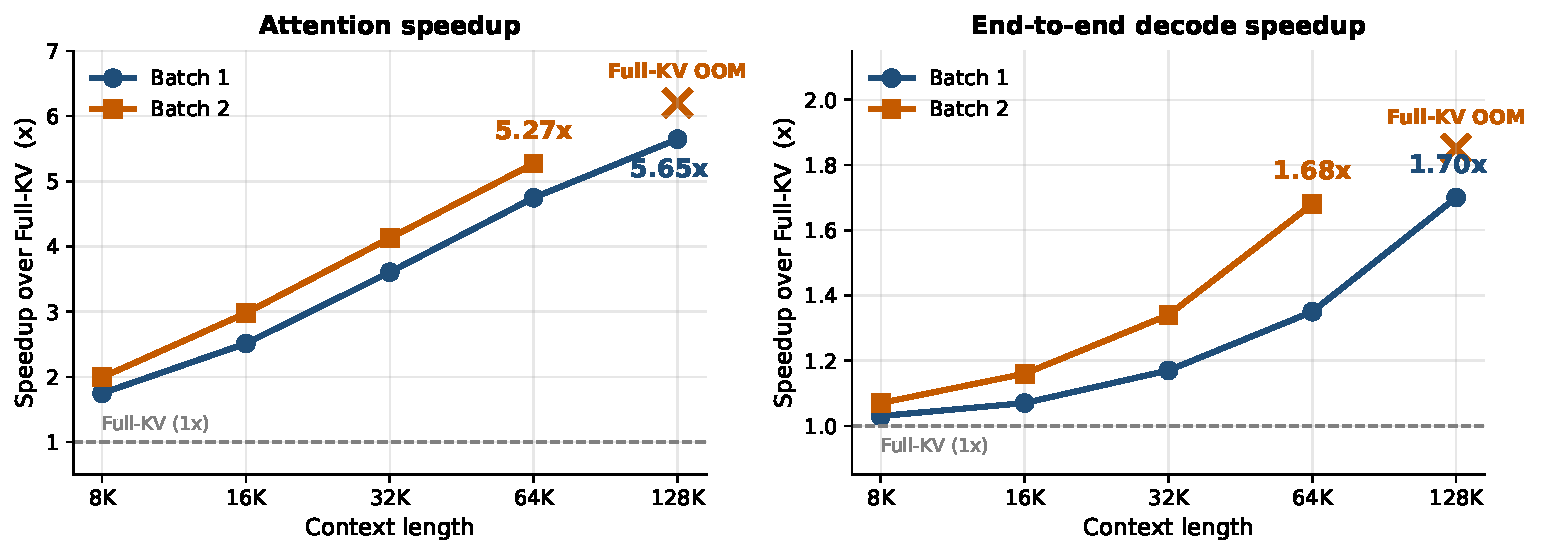
\includegraphics[width=\textwidth]{figures/dct_speedup.pdf}
  \caption[Decode speedup of DCT-Page over Full-KV.]
  {Decode speedup of DCT-Page over Full-KV on a single A6000 with
  Llama-3.1-8B-Instruct.
  Left: attention-only speedup --- up to $5.65\times$ at $128$K
  context (batch 1) and $5.27\times$ at $64$K (batch 2).
  Right: end-to-end decode speedup including MLP and layer-norm ---
  $1.70\times$ at $128$K (batch 1) and $1.68\times$ at $64$K (batch
  2).  ``Full-KV OOM'' marks configurations at which the dense
  baseline exhausts the $48$~GiB device memory.}
  \label{fig:speedup}
\end{figure}

\begin{table}[ht]
  \centering
  \caption[Per-stage decode-time attribution.]
  {Per-stage decode-time attribution at $L = 32{,}768$, batch 1.
   The Full-KV row reports the time spent inside its attention kernel;
   the DCT-Page rows split the equivalent attention-time budget into
   proxy update, page scoring, the fused top-$k$ selection / KV
   assembly kernel, and the final attention kernel.  All values are
   in milliseconds per decode step, averaged over 128 timed steps.
   QKV and output projections are identical between the two paths and
   are excluded.}
  \label{tab:per-stage}
  \small
  \begin{tabular}{l r}
    \toprule
    Stage & Time (ms/step) \\
    \midrule
    Full-KV: attention kernel & 6.400 \\
    \midrule
    DCT-Page: proxy update                          & 0.004 \\
    DCT-Page: page scoring                          & 0.443 \\
    DCT-Page: top-$k$ selection + KV assembly       & 0.312 \\
    DCT-Page: attention kernel                      & 0.630 \\
    \cmidrule(lr){1-2}
    DCT-Page: total                                 & 1.389 \\
    \bottomrule
  \end{tabular}
\end{table}


% =====================================================================
\section{Comparison with Cluster-Based Multipole Attention}\label{sec:results-multipole}
% =====================================================================

Multipole Attention is omitted from the head-to-head accuracy tables
above because its cluster-based decode path lies on a different point
of the accuracy--throughput Pareto frontier than the page-based
methods (Section~\ref{sec:baselines}).
Table~\ref{tab:multipole} reports DCT-Page and Multipole side by side
on each accuracy benchmark and on decode throughput, so that the
trade-off can be read directly.

% Headline claims (from filled-in numbers below):
%   - RULER: Multipole wins by +2.93 pts on Llama, +4.32 pts on Qwen3.
%   - LongBench v1: Multipole +0.30 (Llama) but DCT-Page +0.15 (Qwen3) -- effectively a tie.
%   - LongBench v2: DCT-Page wins both -- +1.79 (Llama), +0.60 (Qwen3).
%   - Throughput @ 32K B1: DCT-Page 38.52 tok/s vs Multipole 7.5 tok/s
%     => DCT-Page is 5.14x faster.
%   - Pareto: Multipole = highest synthetic accuracy, DCT-Page = far
%     better throughput at indistinguishable real-text accuracy.

\begin{table}[ht]
  \centering
  \caption[DCT-Page vs.\ Multipole: accuracy and throughput.]
  {DCT-Page vs.\ Multipole Attention.  RULER and LongBench v1 are
   reported as averages across their respective tasks; LongBench v2
   is reported as overall accuracy.  Decode throughput is the tokens
   per second at $L = 32{,}768$, batch 1, measured under the protocol
   of Section~\ref{sec:speed-protocol}.}
  \label{tab:multipole}
  \footnotesize
  \setlength{\tabcolsep}{5pt}
  \begin{tabular}{l cc cc cc c}
    \toprule
    & \multicolumn{2}{c}{RULER Avg}
    & \multicolumn{2}{c}{LongBench v1}
    & \multicolumn{2}{c}{LongBench v2}
    & Throughput \\
    \cmidrule(lr){2-3} \cmidrule(lr){4-5} \cmidrule(lr){6-7}
    Method
      & Llama & Qwen3
      & Llama & Qwen3
      & Llama & Qwen3
      & (tok/s) \\
    \midrule
    DCT-Page  & 86.26 & 83.72 & 50.27 & \textbf{48.63} & \textbf{30.02} & \textbf{32.01} & \textbf{38.52} \\
    Multipole & \textbf{89.19} & \textbf{88.04} & \textbf{50.57} & 48.48 & 28.23 & 31.41 & 7.50 \\
    \bottomrule
  \end{tabular}
\end{table}


% =====================================================================
\section{Ablations}\label{sec:ablations}
% =====================================================================

We sweep the four DCT-Page hyperparameters that most influence the
accuracy--throughput trade-off, holding all others at the defaults of
Table~\ref{tab:config}.  All sweeps report RULER average accuracy on
Llama-3.1-8B-Instruct at 32K context; the conclusions transfer to
Qwen3-8B and to LongBench (not shown).

\begin{table}[ht]
  \centering
  \caption[Ablation: page size $P$.]
  {Page size $P$ sweep at fixed selected-token budget
   $B \cdot P = 2{,}048$.  Smaller $P$ gives finer selection at the
   cost of more bookkeeping work; larger $P$ amortizes overhead but
   loses selectivity inside the page.}
  \label{tab:abl-page-size}
  \small
  \begin{tabular}{c c c c}
    \toprule
    $P$ & $B$ (pages) & RULER Avg (\%) & Tok/s @ 32K \\
    \midrule
    16  & 128 & & \\
    32  & 64  & & \\
    64  & 32  & & \\
    128 & 16  & & \\
    \bottomrule
  \end{tabular}
\end{table}

\begin{table}[ht]
  \centering
  \caption[Ablation: selected-token budget.]
  {Selected-token budget sweep at fixed $P{=}32$.  $k$ is the
   middle-page count $B - S - R$ at $S{=}1, R{=}4$.}
  \label{tab:abl-budget}
  \small
  \begin{tabular}{c c c c}
    \toprule
    Budget (tokens) & $B$ (pages) & $k$ (middle) & RULER Avg (\%) \\
    \midrule
    1{,}024 &  32 & 27  & \\
    2{,}048 &  64 & 59  & \\
    4{,}096 & 128 & 123 & \\
    \bottomrule
  \end{tabular}
\end{table}

\begin{table}[ht]
  \centering
  \caption[Ablation: compression ratio $C/P$.]
  {Compression ratio sweep at fixed $P{=}32$.  $C$ is the number of
   proxy tokens retained per page (Section~\ref{sec:proxy}).}
  \label{tab:abl-compress}
  \small
  \begin{tabular}{c c c}
    \toprule
    $C$ & $C/P$ & RULER Avg (\%) \\
    \midrule
    1 & $1/32$ & \\
    2 & $1/16$ & \\
    4 & $1/8$  & \\
    8 & $1/4$  & \\
    \bottomrule
  \end{tabular}
\end{table}

\begin{table}[ht]
  \centering
  \caption[Ablation: scoring and GQA-group aggregators.]
  {Choice of proxy-token aggregator $\rho$ and GQA-group aggregator
   $\gamma$ (Section~\ref{sec:scoring}).}
  \label{tab:abl-aggregators}
  \small
  \begin{tabular}{c c c}
    \toprule
    $\rho$ & $\gamma$ & RULER Avg (\%) \\
    \midrule
    $\max$  & $\max$  & \\
    $\max$  & mean    & \\
    mean    & $\max$  & \\
    mean    & mean    & \\
    \bottomrule
  \end{tabular}
\end{table}
